% MDPI Information submission source based on the official 23 July 2026 template.
\documentclass[information,article,submit,oneauthor,pdftex]{Definitions/mdpi}

\firstpage{1}
\makeatletter
\setcounter{page}{\@firstpage}
\makeatother
\pubvolume{1}
\issuenum{1}
\articlenumber{0}
\pubyear{2026}
\copyrightyear{2026}
\datereceived{}
\daterevised{}
\dateaccepted{}
\datepublished{}

\usepackage{amsmath,amssymb}
\usepackage{array}
\usepackage{placeins}
\setlength{\headheight}{20pt}

\newcommand{\cov}{\operatorname{Cov}}

\Title{Prequential Answer-Set Calibration for Temporal Knowledge Graph Forecasting}

\Author{Xinyu Wang $^{1,*}$}
\AuthorNames{Xinyu Wang}
\address{%
$^{1}$ \quad Anhui Institute of Information Technology, Wuhu 241000, China}
\corres{Correspondence: xywang68@iflytek.com}

\abstract{Temporal knowledge graphs support event forecasting, yet ranking metrics do not show whether a model can return answer sets with reliable coverage. Static conformal calibration is attractive for this purpose, but its behavior after a temporal split is uncertain. We compare a rolling prequential margin rule with a static margin rule and three published KGCP score transformations under a timestamp-batched protocol. The study covers ICEWS14 and ICEWS05-15, temporal DistMult and a matched-protocol continuous complex scorer, five seeds, controlled deletion of training facts, and filtered-negative sensitivity. At a 0.90 target and 30\% deletion, rolling coverage ranges from 0.8988 to 0.9002. Its gain over static margin is 0.0798--0.1025, whereas its ICEWS14 contrasts with KGCP Minmax and NegScore are inconclusive. Reliability is costly: rolling sets contain 3818--4307 entities on average and are 1.63--2.22 times larger than KGCP Minmax sets. Multi-answer full-set coverage remains 0.217--0.305 below single-answer coverage. Deletion and negative-sampling effects are mostly small or inconclusive. Recent-history calibration can repair aggregate temporal undercoverage, but it is not uniformly superior and does not resolve the utility or multi-answer problem.}

\keyword{temporal knowledge graph; link forecasting; conformal prediction; prequential evaluation; uncertainty quantification; answer sets; distribution shift}

\begin{document}

\section{Introduction}
\label{sec:introduction}

Temporal knowledge graphs (TKGs) represent time-stamped relations among
entities and are used to forecast future events, interactions, and states. A
typical query asks which entity completes a tuple such as
\((s,r,?,t)\). Modern TKG models are usually compared with filtered mean
reciprocal rank (MRR) and Hits@\(K\) \cite{garciaduran2018sequence,li2021regcn,li2022tirgn,cai2023survey}.
These metrics evaluate ordering, but not whether a returned answer set covers a
recorded correct entity at a stated rate. That distinction matters when a
forecast is passed to a human analyst or a downstream decision rule: a
high-ranking model may still produce unreliable confidence scores, while a
nominally reliable set may be too large to use.

Conformal prediction converts model scores into prediction sets without
requiring a probabilistic model of the labels \cite{vovk2005algorithmic,angelopoulos2023gentle}.
KGCP applies this idea to static knowledge graph embeddings, and CondKGCP studies
predicate-conditional answer sets \cite{zhu2025kgcp,zhu2025condkgcp}. Their
results establish useful static baselines, but temporal forecasting presents a
different information structure: calibration data precede test queries, the
score distribution can change with time, and the labels from a test timestamp
must not be used before all queries at that timestamp have been predicted.
Methods for covariate shift, adaptive conformal inference, and
non-exchangeable data address related settings, but require assumptions or
update rules that should not be silently transferred to TKGs
\cite{tibshirani2019covariate,gibbs2021adaptive,barber2023beyond,farinhas2024nexcrc,wang2025ncpnet}.

This paper asks a focused empirical question: \emph{does calibration on recent,
strictly past TKG scores improve answer-set reliability after a temporal split,
and what does that improvement cost?} We answer it with a timestamp-batched
prequential protocol. A frozen scorer predicts every subject and object query
at time \(t\); only after the complete batch is recorded may its observed labels
enter the calibration history. The study compares static and rolling margin
calibration with the NegScore, Minmax, and Softmax nonconformity transformations
reported by KGCP. These are matched-protocol score-transform baselines, not an
exact reproduction of the KGCP authors' complete training pipeline.

The evaluation was expanded in response to three threats to validity. First,
ICEWS14 is supplemented with the longer ICEWS05-15 event graph. Second,
temporal DistMult is supplemented with a continuous-time complex-valued scorer;
the latter follows a ComplEx-style factorization but is not the official
TComplEx optimizer \cite{yang2015distmult,lacroix2020tcomplex}. Third, filtered
and uniform training negatives are compared in paired sensitivity conditions.
The resulting matrix contains 90 completed seed--deletion conditions, 286,480
timestamp summaries, and 28.6 million query-level records.

The main findings are deliberately bounded. Rolling margin calibration restores
near-nominal aggregate coverage in all four dataset--scorer combinations, but
it does not consistently improve on KGCP Minmax or NegScore on ICEWS14 and it
returns much larger sets. Multi-answer queries remain substantially less likely
than single-answer queries to have every recorded answer covered. Moreover,
controlled deletion of training facts does not significantly worsen static
coverage, and filtered-negative effects are mostly inconclusive. The contribution
is therefore a reliability diagnostic and leakage-controlled evaluation, not a
new distribution-free coverage theorem or a claim of universal superiority.

\section{Related Work}
\label{sec:related}

\textbf{Temporal knowledge graph forecasting.}
TKG completion methods range from temporal sequence encoders and tensor
factorizations to recurrent graph networks
\cite{garciaduran2018sequence,lacroix2020tcomplex,li2021regcn,li2022tirgn}.
Simple history-based methods can remain competitive, which makes careful
protocol design as important as model complexity \cite{gastinger2024repeat,gastinger2024tgb2}.
Our calibration layer consumes a frozen all-entity score vector and does not
alter candidate ordering. It is therefore evaluated across two scorer families
rather than presented as a new forecasting backbone.

\textbf{Calibration and conformal answer sets.}
Post-hoc probability calibration has been studied for neural classifiers and
knowledge graph embeddings \cite{guo2017calibration,safavi2020calibration}.
KGCP introduced conformal answer sets for knowledge graph link prediction using
NegScore, query-wise Minmax, and Softmax score transformations
\cite{zhu2025kgcp}. CondKGCP extended this direction toward
predicate-conditional behavior \cite{zhu2025condkgcp}. APS and RAPS provide
ranked probability-mass prediction sets for classifiers
\cite{angelopoulos2021raps}. We use KGCP's three score transformations as
static baselines under the same split and scorer as our margin rules. RAPS is
retained only as a secondary, validation-selected utility diagnostic because
temporal ordering invalidates an automatic transfer of its exchangeable-data
guarantee.

\textbf{Non-exchangeable calibration.}
Weighted conformal prediction, Adaptive Conformal Inference, and subsequent
non-exchangeable analyses show how coverage can be studied under specific forms
of shift or online feedback
\cite{tibshirani2019covariate,gibbs2021adaptive,barber2023beyond,farinhas2024nexcrc}.
NCPNET addresses non-exchangeable temporal graph neural networks
\cite{wang2025ncpnet}. Our rolling rule is intentionally simpler: it estimates
an empirical quantile from the most recent revealed scores. No likelihood-ratio
weights or test-point mass are used, so we make no finite-sample guarantee under
arbitrary drift.

\section{Problem and Prequential Protocol}
\label{sec:method}

\subsection{Queries, Answer Sets, and Metrics}

Let \(\mathcal{E}\) and \(\mathcal{R}\) denote the closed entity and relation
vocabularies. A TKG contains quadruples \((s,r,o,t)\). An object query is
\(x=(s,r,?,t)\), where ``\(?\)'' marks the entity slot to be predicted; it is
not missing manuscript text. Subject prediction is represented as
\((o,r^{-1},?,t)\). For query \(x\), let \(Y_t(x)\subseteq\mathcal{E}\) be all
recorded answers at timestamp \(t\), and let \(C_t(x)\) be the prediction set.

The primary reliability metric is observed-label coverage,
\[
  \widehat{\cov}_{\mathrm{label}}
  =\frac{1}{N}\sum_{(x,y)}\mathbb{1}\{y\in C_t(x)\}.
\]
This label-marginal quantity differs from full-set query coverage,
\(\mathbb{1}\{Y_t(x)\subseteq C_t(x)\}\). We report both, together with mean
set size and filtered MRR. For multi-answer queries, partial answer recall is
\(|Y_t(x)\cap C_t(x)|/|Y_t(x)|\). Coverage always refers to recorded benchmark
labels, not to all events that may be true in the world.

\subsection{Static and Rolling Calibration}

Let \(f_\theta(x,y)\) be a score from a frozen TKG model. Margin nonconformity is
\[
  a_{\mathrm{margin}}(x,y)=\max_{z\in\mathcal{E}} f_\theta(x,z)-f_\theta(x,y),
  \qquad
  C_q(x)=\{y:a_{\mathrm{margin}}(x,y)\le q\}.
\]
For calibration scores \(a_1,\ldots,a_n\) and target \(1-\alpha\), the
finite-sample threshold is the order statistic with index
\(\min\{n,\lceil(n+1)(1-\alpha)\rceil\}\). Static margin estimates this
threshold once from the final initial-calibration interval. Rolling margin
re-estimates it at each test timestamp from the most recent \(W=1000\) scores
that were revealed strictly before that timestamp.

The KGCP baselines use the same frozen score tensors and the same static
calibration interval. For candidate score vector \(f\), their nonconformity
scores are
\[
\begin{aligned}
 a_{\mathrm{Neg}}(y)&=-f_y,\\
 a_{\mathrm{Minmax}}(y)&=-\frac{f_y-\min_z f_z}{\max_z f_z-\min_z f_z},\\
 a_{\mathrm{Softmax}}(y)&=1-\frac{\exp(f_y/T)}{\sum_z\exp(f_z/T)},
\end{aligned}
\]
with zero-range Minmax vectors mapped to zero and \(T=1\). We use the published
score definitions but retrain neither the original KGCP models nor their exact
optimizer. Accordingly, the comparisons isolate score transformation and
temporal updating under one protocol.

At test timestamp \(t\), every query is scored and every set is stored before
any label from \(t\) is revealed. The complete batch is then appended to the
rolling pool. This batch boundary prevents within-timestamp leakage.

\subsection{What the Empirical Threshold Does and Does Not Guarantee}

Condition on the frozen scorer and all information available before timestamp
\(t\). Let \(F_t\) be the CDF of the current label's nonconformity score. Let
\(H_{t,w}\) be the population mixture represented by a weighted calibration
pool and \(\widehat H_{t,w}\) its empirical CDF. Define
\[
  \delta_t=\sup_u|F_t(u)-H_{t,w}(u)|,\qquad
  \epsilon_t=\sup_u|\widehat H_{t,w}(u)-H_{t,w}(u)|,
\]
and let \(\eta_t\) be the largest total empirical weight assigned to scores
tied at one value.

\noindent\textbf{Proposition 1 (set geometry).}\quad
For nonnegative \(q_1\le q_2\), \(C_{q_1}(x)\subseteq C_{q_2}(x)\) and
\(C_{q_1}(x)\neq\varnothing\). Moreover,
\(Y_t\in C_{q_t}(X_t)\) if and only if the observed-label nonconformity score is
at most \(q_t\).

\emph{Proof.}
The set is a nonconformity sublevel set and therefore grows with the threshold.
The top-scoring entity has margin zero. The final statement follows directly
from the definition of \(C_q\). \hfill\(\square\)

\noindent\textbf{Proposition 2 (deterministic coverage decomposition).}\quad
For the inclusive empirical threshold at level \(1-\alpha\),
\[
  1-\alpha-\delta_t-\epsilon_t
  \le F_t(q_t)\le
  1-\alpha+\delta_t+\epsilon_t+\eta_t,
  \tag{1}\label{eq:coverage-decomposition}
\]
with either side clipped to \([0,1]\).

\emph{Proof.}
The empirical CDF is at least \(1-\alpha\) at the inclusive quantile, so the
population history CDF is at least \(1-\alpha-\epsilon_t\), and the current CDF
is at least a further \(\delta_t\) below. Immediately before the quantile, the
empirical CDF is below \(1-\alpha\); its jump is at most \(\eta_t\). Applying
the same two sup-norm deviations gives the upper bound. \hfill\(\square\)

Equation~\eqref{eq:coverage-decomposition} is a decomposition, not a new
distribution-free guarantee. A shorter history may reduce temporal mismatch
\(\delta_t\), while increasing estimation error or tie mass. The experiments
measure the resulting reliability--utility trade-off rather than assuming that
recent history must be better.

\section{Experimental Design}
\label{sec:experiments}

\subsection{Data, Scorers, and Conditions}

ICEWS14 and ICEWS05-15 are event knowledge graph benchmarks derived from the
ICEWS coded event data \cite{boschee2015icews}. Table~\ref{tab:data} reports the
normalized graph sizes. Unique timestamps are sorted: the earliest 60\% train
the scorer, the next 20\% provide four disjoint validation and calibration
roles, and the final 20\% form the test stream. The middle interval is divided
chronologically into 25\% scorer validation, 30\% calibrator tuning, 15\%
selector validation, and 30\% final initial calibration.

\begin{table}[t]
\centering
\caption{Normalized dataset statistics. Relations exclude the inverse copies
added internally for subject prediction.\label{tab:data}}
\begin{tabular}{lrrrr}
\toprule
Dataset & Entities & Relations & Facts & Timestamps\\
\midrule
ICEWS14 & 7,128 & 230 & 90,730 & 365\\
ICEWS05-15 & 10,488 & 251 & 461,329 & 4,017\\
\bottomrule
\end{tabular}
\end{table}

Temporal DistMult uses 256-dimensional real embeddings. The second scorer uses
128-dimensional complex embeddings and a shared continuous time map formed from
constant, linear, quadratic, sine, and cosine features. It is a
matched-protocol ComplEx-style alternative, not an exact implementation of the
discrete-time TComplEx training procedure. Both scorers use the same pairwise
softplus objective, Adam, learning rate \(10^{-3}\), weight decay \(10^{-6}\),
batch size 1024, 128 negatives, at most 200 epochs, and validation-based early
stopping.

The primary matrix uses filtered training negatives and five seeds
\(\{17,29,43,59,71\}\). ICEWS14 is evaluated with both scorers at deletion
rates \(\{0,0.1,0.2,0.3\}\); ICEWS05-15 uses all four rates for DistMult and
rates \(\{0,0.3\}\) for the complex scorer. Deletion affects training facts
only. It is seeded and uniform subject to retaining each entity's earliest
training occurrence when deletion would otherwise remove every occurrence.
Uniform-negative sensitivity is evaluated at rates 0 and 0.3 for ICEWS05-15
DistMult and ICEWS14 continuous ComplEx. Filtered negatives exclude positives
retained in the training graph; they do not use future facts.

\subsection{Inference and Reproducibility}

The target coverage is 0.90. Primary uncertainty intervals use 20,000
equal-seed circular moving-block bootstrap replicates with a seven-timestamp
block; lengths 3, 14, and 21 are sensitivity checks. Paired contrasts reuse the
same seed and timestamp blocks. The analysis reports coverage, mean set size,
filtered MRR, full-set query coverage, and partial answer recall. The complete
code, resolved configurations, paper data, figure-generation scripts, checksums,
and release audit are available at
\url{https://github.com/xywang815/riskcal-tkg-w}. Raw ICEWS data are obtained
from \url{https://doi.org/10.7910/DVN/28075} and the public benchmark archive
documented in the repository.

OpenAI Codex was used to assist code development, experiment orchestration,
language editing, and document formatting. The author reviewed the source,
verified the checksum-bound outputs, and takes responsibility for the analyses,
figures, and manuscript.

\section{Results}
\label{sec:results}

All 90 planned seed--deletion conditions completed. The evidence contains
286,480 timestamp rows and 28,626,600 query-label rows, including 4,858,050
rows from multi-answer queries. No incomplete condition or pilot result is used
below.

\subsection{Coverage Generalizes, but the Best Static Baseline Depends on the Dataset}

Figure~\ref{fig:generalization} shows observed-label coverage. At 30\% deletion,
rolling margin obtains 0.8996 and 0.8988 on ICEWS14 with DistMult and continuous
ComplEx, and 0.9002 with both scorers on ICEWS05-15. Relative to static margin,
the corresponding gains are 0.0798 (95\% CI [0.0621, 0.0999]), 0.0802
([0.0612, 0.1012]), 0.1011 ([0.0921, 0.1102]), and 0.1025
([0.0937, 0.1111]). KGCP Softmax behaves similarly to static margin and also
under-covers in all four settings.

\begin{figure}[t]
\centering
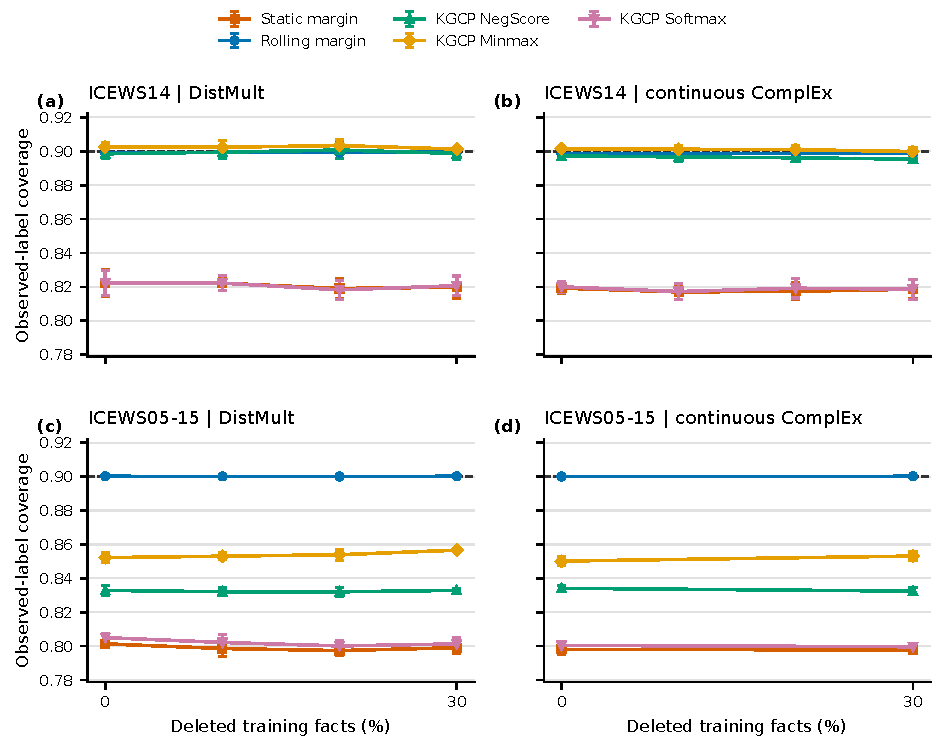
\includegraphics[width=\textwidth]{figures/expansion/expansion_generalization.pdf}
\caption{Observed-label coverage across deletion rates. Points are means over
five seeds and error bars are one seed standard deviation; the dashed line is
the 0.90 target. ICEWS05-15 continuous ComplEx was evaluated at 0 and 30\%
deletion. All methods use the same scorer within a panel.\label{fig:generalization}}
\end{figure}

The comparison with stronger KGCP transformations is heterogeneous. On
ICEWS05-15, rolling margin exceeds KGCP Minmax by 0.0436 ([0.0387, 0.0486])
with DistMult and 0.0471 ([0.0418, 0.0524]) with continuous ComplEx; its gains
over KGCP NegScore are 0.0673 and 0.0678. On ICEWS14, however, the
rolling-minus-Minmax intervals are [-0.0074, 0.0042] and [-0.0072, 0.0058],
and the NegScore intervals also cross zero. KGCP Minmax and NegScore already
reach approximately nominal coverage there. Rolling calibration is therefore a
robust temporal repair relative to the two under-covering static rules, not a
uniform improvement over all KGCP scores.

\subsection{Near-Nominal Coverage Requires Large Sets}

At 30\% deletion, rolling mean set sizes are 3,870.6 and 3,818.0 entities on
ICEWS14 and 4,307.2 and 4,260.1 on ICEWS05-15 for DistMult and continuous
ComplEx, respectively. These sets are 1.63--2.22 times larger than KGCP Minmax
sets and 1.41--1.85 times larger than static-margin sets. On ICEWS14, KGCP
Minmax reaches nominal coverage with substantially smaller sets than rolling
margin. On ICEWS05-15, rolling margin is more reliable than KGCP Minmax but pays
for that gain with more than twice the mean set size. These results define a
reliability--utility frontier rather than a single winning method.

\subsection{Deletion and Negative Sampling Do Not Explain the Main Effect}

Figure~\ref{fig:diagnostics} separates method contrasts from two stress tests.
For 30\% minus 0\% deletion, every static-margin and rolling-margin coverage
interval includes zero. Static changes range from -0.0024 to -0.0004, and
rolling changes range from 0.0000 to 0.0005. The experiment therefore does not
support the claim that deleted training facts cause static calibration failure.
Deletion remains a controlled scorer stress, while temporal mismatch is the
more defensible motivation.

Filtered-minus-uniform rolling effects also include zero in all four paired
conditions. A small positive static-margin effect appears only for ICEWS05-15
DistMult without deletion (0.0020 [0.0005, 0.0038]); the other static intervals
cross zero. The main coverage conclusions are not driven by the tested negative
sampling choice.

\begin{figure}[H]
\centering
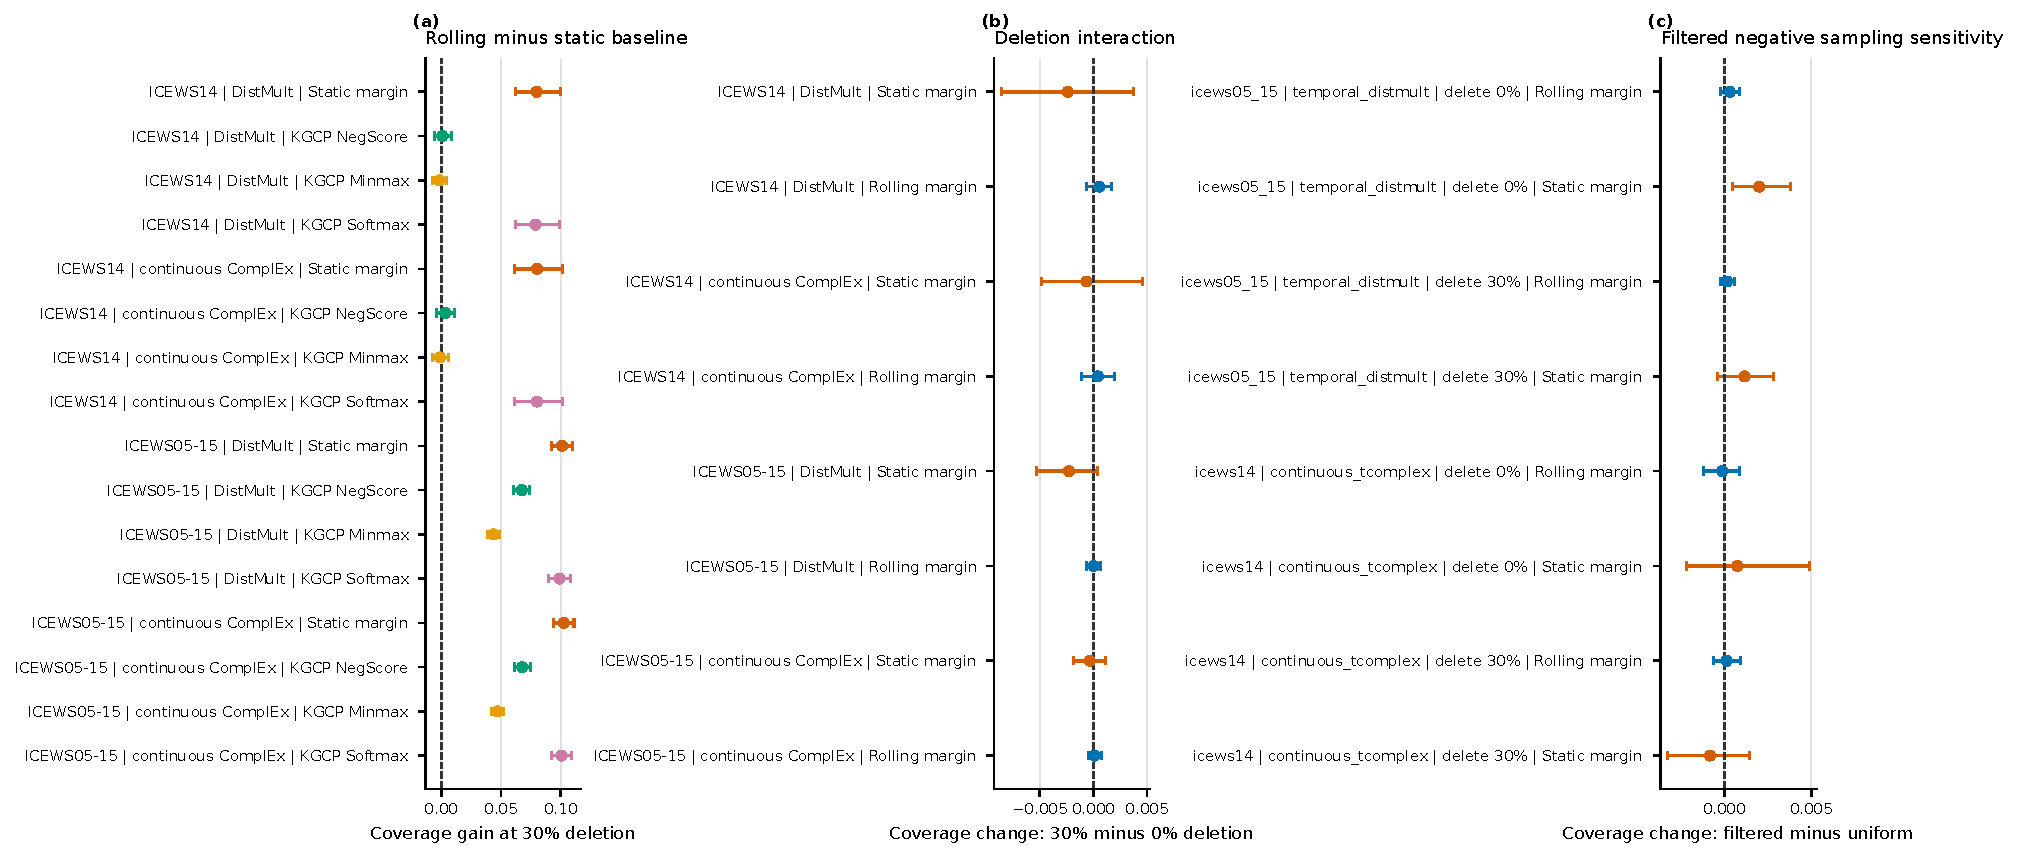
\includegraphics[width=\textwidth]{figures/expansion/expansion_reviewer_diagnostics.pdf}
\caption{Paired timestamp-block bootstrap diagnostics (20,000 replicates,
seven-timestamp blocks). (\textbf{a}) Rolling-minus-static coverage at 30\%
deletion. (\textbf{b}) Coverage change caused by 30\% training-fact deletion.
(\textbf{c}) Coverage change from filtered rather than uniform training
negatives. Intervals crossing zero are inconclusive.\label{fig:diagnostics}}
\end{figure}

\subsection{Multi-Answer Queries Remain a Failure Mode}

Label-marginal coverage can hide whether a set contains every answer to a query.
At 30\% deletion, rolling full-set coverage for multi-answer queries is 0.2792
below single-answer coverage on ICEWS14 DistMult, with a 95\% interval of
[-0.2992, -0.2600]. The gaps are -0.3054 on ICEWS14 continuous ComplEx,
-0.2174 on ICEWS05-15 DistMult, and -0.2294 on ICEWS05-15 continuous ComplEx
(Figure~\ref{fig:multi}). For example, ICEWS14 DistMult rolling coverage is
0.6532 for multi-answer queries and 0.9305 for single-answer queries. Rolling
calibration narrows the gap relative to static margin and KGCP Softmax, but does
not remove it.

\begin{figure}[H]
\centering
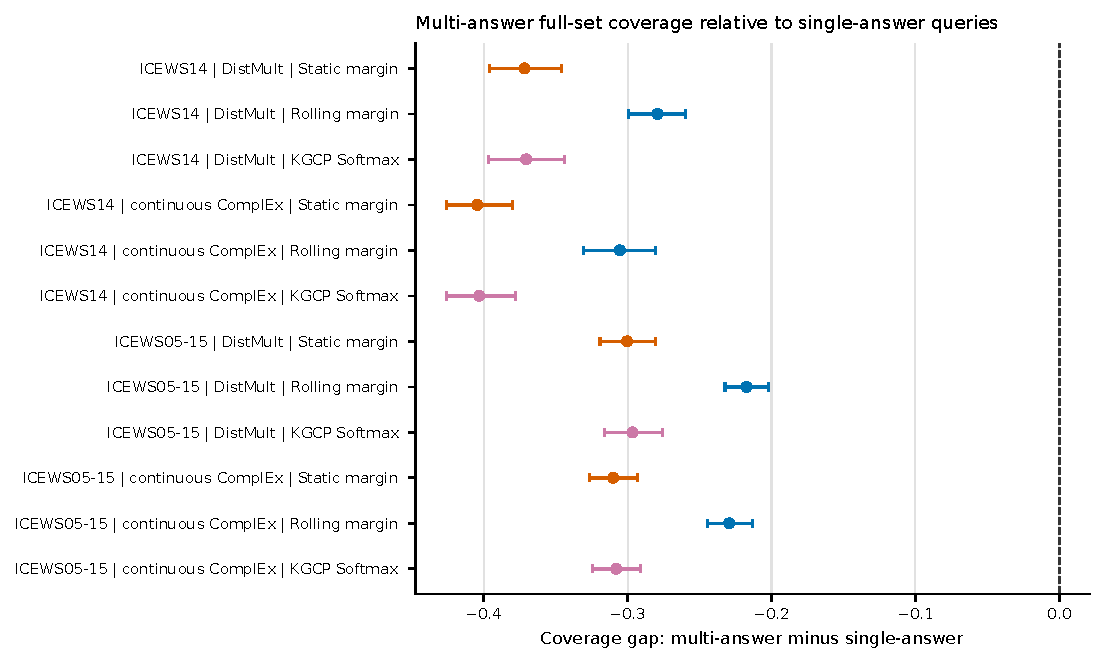
\includegraphics[width=0.96\textwidth]{figures/expansion/expansion_multi_answer.pdf}
\caption{Full-set coverage for multi-answer queries minus full-set coverage for
single-answer queries at 30\% deletion. Points are paired estimates and bars are
95\% timestamp-block bootstrap intervals. More negative values indicate a
larger multi-answer deficit.\label{fig:multi}}
\end{figure}

\section{Discussion and Conclusions}
\label{sec:discussion}

The experiments answer the central question with a qualified yes. Updating a
margin threshold from strictly past scores restores aggregate coverage near
0.90 across two ICEWS datasets and two scorer families. The same conclusion is
not obtained by choosing a different static score alone on ICEWS05-15, where
all three KGCP transformations remain below target. On ICEWS14, however, KGCP
Minmax and NegScore already perform near the target with smaller sets. The
appropriate operational choice therefore depends on the dataset and on the
cost assigned to missed labels versus large candidate sets.

The negative results narrow the paper's contribution. Training-fact deletion
does not materially worsen static coverage, so it cannot serve as the causal
explanation for miscalibration. Filtered training negatives also have little
effect on coverage in the paired tests. Both interventions are useful robustness
checks, but neither supports a broad mechanism claim. The stable pattern is the
difference between an early fixed threshold and a recent-history threshold
under temporal ordering.

The multi-answer diagnostic is more serious. A method can attain nominal
label-marginal coverage while failing to include all recorded answers for many
queries. This gap is partly semantic: each additional valid label makes the
full-set event harder. It is also practical, because multi-answer queries often
represent the cases in which a shortlist is most valuable. Future methods
should calibrate query-level set coverage or structured answer recall directly,
rather than treating repeated query labels as independent examples.

Several limitations remain. ICEWS14 and ICEWS05-15 are related political-event
graphs, not a broad sample of temporal graph domains. The continuous complex
scorer is a matched-protocol implementation and not the official TComplEx
optimizer or checkpoint. Similarly, the KGCP baselines reproduce published
score transformations under a common static calibration split, not the complete
original pipeline. Five seeds limit training-randomness inference, while the
moving-block bootstrap only approximates temporal dependence. Exact
all-entity scoring also becomes expensive for substantially larger vocabularies.

In practice, rolling calibration is useful as an audit and repair when recent
labels arrive before the next prediction batch. It should not be deployed by
coverage alone: mean and tail set size, feedback delay, relation-side behavior,
and multi-answer full-set coverage must be examined together. Future work should
test official and recurrent TKG backbones, non-event and inductive datasets,
predicate-conditional temporal calibration, and compact structured sets with
explicit multi-answer objectives.

In conclusion, recent-history prequential calibration can correct aggregate
temporal undercoverage, but the improvement is baseline-dependent and often
requires thousands of candidate entities. The present evidence supports a
transparent reliability--utility diagnostic. It does not support universal
superiority, a deletion-driven failure mechanism, or a distribution-free
coverage guarantee under arbitrary temporal drift.

\authorcontributions{Conceptualization, X.W.; methodology, X.W.; software, X.W.; validation, X.W.; formal analysis, X.W.; investigation, X.W.; data curation, X.W.; writing--original draft preparation, X.W.; writing--review and editing, X.W.; visualization, X.W.; project administration, X.W.; funding acquisition, X.W. The author has read and agreed to the published version of the manuscript.}

\funding{This research was funded by the Natural Science Research Project of Universities in Anhui Province, grant number 2023AH052916.}

\institutionalreview{Not applicable.}

\informedconsent{Not applicable.}

\dataavailability{The study uses ICEWS14 and ICEWS05-15 derived from the public ICEWS Coded Event Data at \url{https://doi.org/10.7910/DVN/28075}. Source code, preprocessing scripts, resolved configurations, derived result tables, figure-generation scripts, checksums, and the clean-clone release audit are available at \url{https://github.com/xywang815/riskcal-tkg-w} under the MIT License. The submission snapshot is identified by the tag \texttt{v1.0.0-mdpi-information-\allowbreak submission}.}

\conflictsofinterest{The author declares no conflicts of interest. The funder had no role in the design of the study; in the collection, analysis, or interpretation of data; in the writing of the manuscript; or in the decision to publish the results.}

\FloatBarrier
\reftitle{References}
\externalbibliography{yes}
\bibliography{references}

\end{document}
